\subsection*{\revise{NSC in the retina and visual cortex}}

\revise{Due to its roots in efficient-coding theories of natural image processing,
\ac{NSC} figures prominently in the vision neuroscience literature.}

\revise{For example, \ac{NMF}-based models were able to reconstruct
\emph{in vitro} neuronal spike trains from the salamander retina 
\cite{Onken2016,Liu2017}.
By combining spike-triggered average with \ac{NMF},
Liu and colleagues \cite{Liu2017} were able to identify the subunit layout
of retinal ganglion cells
(Fig.~\ref{fig:NMF|retina}).
Whereas modules were constrained to be have nonnegative elements,
stimuli were represented by their contrast values (i.e., their relative deviation from mean light intensity, which could be positive or negative).
The goal of their \ac{NMF} variant was then to seek weights and nonnegative modules
that minimize the difference, in a least-squares sense, between the spike-triggered
stimuli and the reconstruction.
Interestingly, the identified subunits corresponded to 
individual presynaptic bipolar cells,
as verified by multielectrode array recordings with simultaneous recordings from
individual bipolar cells through sharp microelectrodes \cite{Liu2017}.
This allowed the researchers to improve predictions about how ganglion cells respond
to natural stimuli, without the need to guess a specific model structure that may be constrained in terms of the size, shape, number, or nonlinearity of 
ganglion cell subunits.}

\begin{figure}[!b]
	\centering
	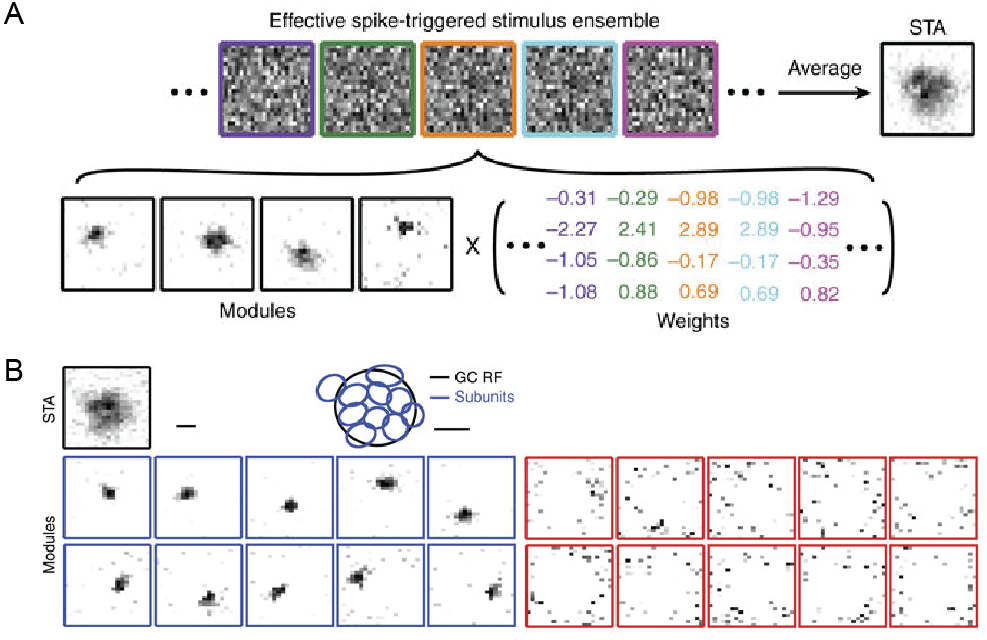
\includegraphics[width=\textwidth]{fig-rev1-retina}
    \caption{
    \revise{Identification of retinal ganglion cell subunits 
    with \ac{STNMF} (adapted from \cite{Liu2017}).
    \textbf{\emph{A}},
	     Samples of a ganglion cell’s effective spike-triggered stimulus ensemble (top),
         whose average corresponds to the cell’s \ac{STA}.
         For easier visual comparison with the subunits,
         \acp{STA} are displayed with negative pixel values set to zero and
         with zero corresponding to white in the grayscale image.
         \ac{STNMF} decomposes this ensemble into a set of modules and 
         a weight matrix (bottom).
         The example here shows four modules that were identified for
         a sample ganglion cell.
    \textbf{\emph{B}},
         Modules obtained for another sample ganglion cell by applying \ac{STNMF}
         with 20 modules (bottom 2 rows). Some modules have a strongly localized structure 
         (blue frames), others are more noise-like (red frames).
         The top row shows the cell’s receptive field,
         given by the spatial component of the STA, as well as the fitted \ac{RF} outline
         (GC RF, black ellipse), together with outlines of the localized subunits 
         (blue ellipses). Scale bars, 100 µm.
    }}
	\label{fig:NMF|retina}
\end{figure}

\revise{As mentioned in the previous section,
\ac{NSC} has been extensively applied to early visual cortex,
where it has successfully explained 
orientation and frequency tuning of simple and complex cells in \ac{V1} \cite{Hoyer2003},
edge-like pooling of spatial frequency channels in V1 \cite{Hyvarinen2005},
including \ac{RF} properties such as end-stopping and contour integration 
\cite{HoyerHyvarinen2002}.
With the exception of face processing in \ac{IT}
\cite{LeeSeung1999,ChangTsao2017},
\ac{NSC} has yet to be applied to higher-order areas in the ventral visual stream.
The success of \ac{NSC} in explaining V1 and V2 response properties
suggests that it might be possible to extend the model to texture integration in
V4.}


\begin{figure}[!b]
	\centering
	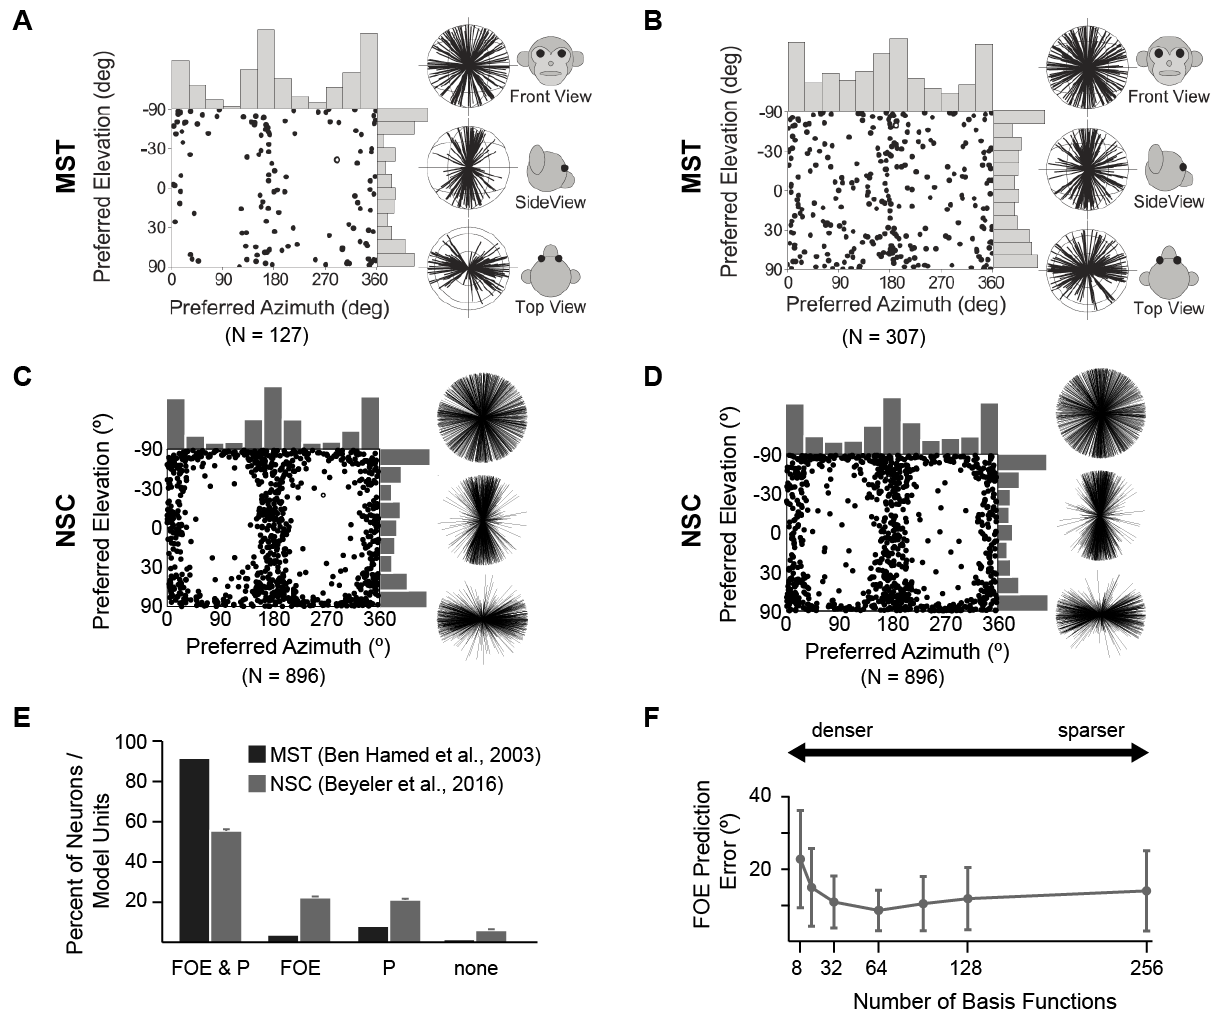
\includegraphics[width=0.97\textwidth]{fig-rev1-MST}
    \caption{
    \revise{
    \textbf{\emph{A-D}},
         Distribution of 3D direction preferences of macaque \ac{MSTd} neurons
         (rotation, \textbf{\emph{A}}; translation, \textbf{\emph{B}}; 
         reprinted from \cite{Takahashi2007})
         and model units in the \ac{NSC}-based sparse decomposition model
         (rotation, \textbf{\emph{C}}; translation, \textbf{\emph{D}}; 
         reprinted from \cite{Beyeler2016}).
         Each data point in the scatter plots corresponds to the preferred azimuth
         (abscissa) and elevation (ordinate) of a single neuron.
         Histograms along the top and right sides of each scatter plot show the
         marginal distributions.
         Also shown are 2D projections (front view, side view, and top view)
         of unit-length 3D preferred direction vectors (each radial line represents
         one neuron).
    \textbf{\emph{E}},
         Distribution of focus of expansion (FOE) and pursuit (P) selectivities
         in macaque \ac{MSTd} (dark gray) and model \ac{MSTd} (light gray;
         reprinted from \cite{Beyeler2016}).
         Neurons or model units were involved in encoding heading (FOE),
         eye velocity (P), both (FOE \& P), or neither (none).
    \textbf{\emph{F}},
         Heading prediction (generalization) error as a function of the
         number of basis functions using 10-fold cross-validation.
         Vertical bars are the SD (reprinted from \cite{Beyeler2016}).
    }}
	\label{fig:NMF|MSTd}
\end{figure}

\revise{In our own work, we found evidence for \ac{NSC} in the dorsal visual stream.
Specifically, we demonstrated that simulated neurons 
in a \ac{NSC} based model of \ac{MSTd} 
responded to  large optic flow fields in much the same way as real neurons in macaque \ac{MSTd} \cite{Beyeler2016}.
Fig.~\ref{fig:NMF|MSTd} shows the distribution of direction preferences
of \ac{MSTd} cells (Fig.~\ref{fig:NMF|MSTd}A, B; \cite{Takahashi2007})
and \ac{MSTd}-like model units (Fig.~\ref{fig:NMF|MSTd}C, D; \cite{Beyeler2016})
for visual translation and rotation.
Each data point in the scatter plots specifies the preferred 3D direction
of a single neuron or model unit.
Histograms along the boundaries show the marginal distributions of azimuth
and elevation preferences.}
Not only did individual units match response properties of individual neurons
in macaque \ac{MSTd},
but the model was able to recover statistical properties of the \ac{MSTd}
population as a whole, such as a relative overrepresentation of lateral
headings (Fig.~\ref{fig:NMF|MSTd}C, D).

\revise{\ac{MSTd} is known to encode a number of perceptual variables,
such as the direction of travel (heading) and eye rotation velocity.
During forward movement, retinal flow radiates out symmetrically from a single point,
the focus of expansion (FOE), from which heading can be inferred.
However, instead of consisting of a set of distinct subpopulations,
each specialized to encode a particular perceptual variable,
\ac{MSTd} has been found to consist of neurons that act more like basis functions,
where a majority of cells were involved in the simultaneous encoding of multiple
perceptual variables (Fig.~\ref{fig:NMF|MSTd}E).
A similar picture emerged when we investigated the involvement of \ac{MSTd}-like
model units in the encoding of both heading and eye rotation velocity
(Fig.~\ref{fig:NMF|MSTd}E).}

\revise{Interestingly, the sparsity regime in which model \ac{MSTd} achieved the
lowest heading prediction error (Fig.~\ref{fig:NMF|MSTd}F) was also the
regime in which \ac{MSTd}-like model units reproduced a variety of known
\ac{MSTd} visual response properties
(for experimental details refer to \cite{Beyeler2016}).
In contrast to findings about early visual cortex,
this regime does not use an overcomplete basis set \cite{OlshausenField1996},
yet can still be considered a sparse coding regime \cite{SpanneJorntell2015}.
Such an intermediary sparse code might be better suited
(as opposed to an overcomplete basis set)
for areas such as \ac{MSTd},
because the increased memory capacity of such a code might lead to compact
and multifaceted encodings of various perceptual variables
\cite{BenHamed2003}.}




\subsection*{\revise{NSC in the auditory cortex}}

\revise{The auditory cortex is a prime example of efficient coding. The auditory system is believed to decompose auditory signals into
a set of elementary acoustic features \cite{SmithLewicki2006},
such that the complete acoustic waveform can be described by a
sparse population code that operates near an information-theoretic optimum
\cite{SmithLewicki2006,rokem2006,Hromadka2008}.
It is therefore not surprising that computational models based on \ac{NSC}
have been very successful at describing the spectro-temporal \acp{RF}
of neurons in the \ac{A1} \cite{Martinez2015,David2007}.
Response properties of \ac{A1} neurons are well described by a spectrogram;
they are often tuned to stimulus frequency but are rarely phase-locked
to oscillations of the sound waveform \cite{Leaver2010}.
The cortical representation of auditory signals seems to not only be sparse,
but also rely on statistically independent acoustic features \cite{Klein2003}.}

\revise{Similar to visual cortex, auditory cortex is hierarchically organized,
with neurons in \ac{A1} responding to simple acoustic features of natural sounds,
and higher-order areas responding to more behaviorally relevant stimuli.
The anterior superior temporal region of auditory cortex, for example,
responds to categories of acoustic objects,
such as sounds produced by voices and musical instruments
\cite{Leaver2010}.
An intriguing question for future modeling studies is therefore 
whether \ac{NSC} can be extended to the next level of the auditory hierarchy:
Would it be possible to construct more complex acoustic objects from a sparse,
parts-based set of elementary, \ac{A1}-like acoustic features?
And would the representation of such acoustic objects resemble neuronal responses
in the anterior superior temporal region of auditory cortex?}

% \revise{The primary auditory cortex
% % similar to the early visual cortex and somatosensory cortex,
% % \mikeNote{A1 is actually higher up in the auditory hierarchy than V1 is in the visual hierarchy. I think the same is true for S1. Confusing to compare them}
% may also feature parts-based representations, hinted at by the tonotopic organization of the region, which been determined through multiple neuroimaging studies in humans, as well as in electrophysiological recordings in nonhuman primates \cite{humphries2010,bendor2008}. This functional organization is reminiscent of the organization of early visual cortex. Likewise, studies of auditory cortex support a hierarchically organized pathway, with more complex acoustic objects represented higher up the hierarchy. In support of this idea, the anterior superior temporal region of auditory cortex exhibits sensitivity to categories of acoustic objects (such as sounds produced by voices or by musical instruments), while neurons in regions that are closer to the primary auditory cortex operate more like feature detectors, responding to acoustic features of natural sounds 
% \cite{Leaver2010}. Additionally, sparse coding for vocalizations has been found in the primary auditory cortex of marmoset monkeys, supporting the usage of sparse coding principles for behaviorally relevant sounds \cite{Terashima2013}.}


% \revise{The auditory cortex seems to rely on precise spike timing for efficient information transmission based on experiments that have examined the stimulus-response joint probability distribution in grasshoppers. Findings suggest that the information transmission rate of auditory receptor neurons increase with the amplitude modulation of a stimulus. Furthermore, naturalistic stimuli were encoded suboptimally as compared to idealized Gaussian stimuli, suggesting that auditory receptor neurons encode specific behaviorally relevant stimulus features, consistent with a system that is minimizing metabolic energy costs \cite{rokem2006}. Another finding from awake, behaving rats confirms the sparse population representation of sounds and found that fewer than 5\% of neurons were active at any given time, with most stimuli eliciting high firing rates, but some eliciting very low firing rates in some neurons \cite{Hromadka2008}.}

% \begin{figure}[!h]
% 	\centering
% 	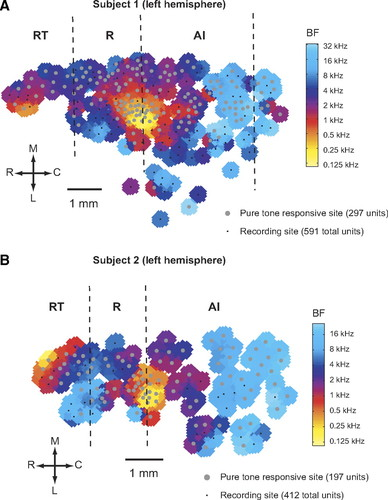
\includegraphics[width=\textwidth]{auditoryTonotopic}
%     \caption{\revise{Reproduced from Bendor et al. 2008 \cite{bendor2008}. Tonotopic organization of neuronal responses to tones of varying frequency in two marmomset monkeys. AI = primary auditory cortex, R = rostral field, and RT = rostrotemporal field. These primary fields are referred to as the `core regions' of auditory cortex. They are heavily interconnected and receive input from one another and from the thalamus, which supports tonotopic organization. The presentation of low to high frequency tones of varying purity results in a gradient of frequency sensitivity across the three fields.}}
% 	\label{fig:auditoryTonotopic}
% \end{figure}

% \revise{The primary auditory cortex
% % similar to the early visual cortex and somatosensory cortex,
% % \mikeNote{A1 is actually higher up in the auditory hierarchy than V1 is in the visual hierarchy. I think the same is true for S1. Confusing to compare them}
% may also feature parts-based representations, hinted at by the tonotopic organization of the region, which been determined through multiple neuroimaging studies in humans, as well as in electrophysiological recordings in nonhuman primates \cite{humphries2010,bendor2008}. This functional organization is reminiscent of the organization of early visual cortex. Likewise, studies of auditory cortex support a hierarchically organized pathway, with more complex acoustic objects represented higher up the hierarchy. In support of this idea, the anterior superior temporal region of auditory cortex exhibits sensitivity to categories of acoustic objects (such as sounds produced by voices or by musical instruments), while neurons in regions that are closer to the primary auditory cortex operate more like feature detectors, responding to acoustic features of natural sounds 
% \cite{Leaver2010}. Additionally, sparse coding for vocalizations has been found in the primary auditory cortex of marmoset monkeys, supporting the usage of sparse coding principles for behaviorally relevant sounds \cite{Terashima2013}.}



\subsection*{\revise{NSC in the olfactory cortex}}

\revise{In contrast to most other sensory modalities, 
the basic perceptual dimensions of olfaction remain unclear.
Odors evoke complex responses in granule cells (located in the olfactory bulb)
that evolve over hundreds of milliseconds \cite{Broome2006}.
Granule cells use a sparse combinatorial code to convey information about odor identity
and concentration \cite{Koulakov2011,Gupta2015}.
% \revise{ The segregated odor mapping contained in the olfactory bulb is then transmitted to the piriform cortex (considered specialized for olfaction), which is thought to be where odor object percepts are formed \cite{chen2014,stettler2009}. The piriform cortex does not exhibit a topographic organization scheme (thus there is no clustered or graded pattern of response that can be mapped), but neurons in this region nonetheless elicit unique but overlapping ensemble-based responses to odorants \cite{stettler2009}. However, a spatial structure can be discerned when examining the projections of output neurons in the piriform cortex, which are highly segregated and functionally specific \cite{chen2014}.}
Downstream from the olfactory bulb, odors tend to activate a small but consistent
proportion ($\sim 10\%$) of cortical neurons in the piriform cortex \cite{poo2009},
which is thought to form odor object percepts \cite{chen2014,stettler2009}.
% \revise{In rat piriform cortex, odors evoke sparse ensemble activity across the population that results from an imbalance between excitation and inhibition (excitation is uncommon and odor-specific, while inhibitory responses are widespread and broadly tuned) \cite{poo2009}, a finding that is also observed in awake, behaving mice \cite{rinberg2006}. Odors tend to activate a small but consistent proportion of cortical neurons in the piriform cortex (9 to 11\%). Furthermore, olfactory cortical neurons responded selectively to stimuli, and population responses to odors were very sparse, providing evidence for both lifetime and population sparseness in the olfactory cortex \cite{poo2009}.}
% \mikeNote{we don't want to anger reviewer  with population sparseness}
Although piriform cortex is not topographically organized,
a spatial structure can be discerned when examining the projections of output neurons,
which are highly segregated and functionally specific.
Whereas the anterior piriform cortex is associated with the encoding of 
odor identity and odor structure, 
the posterior piriform cortex is involved in associational aspects of odors, 
such as valence and similarity \cite{chen2014,gottfried2006}.}
% \revise{It has also been observed that the anterior and posterior piriform cortex are differentially involved in odor processing. The anterior piriform cortex is associated with the encoding of odor identity and odor structure, while the posterior piriform cortex is involved in associational aspects of odor, such as valence and similarity \cite{chen2014,gottfried2006}. The olfactory bulb and piriform cortex also seem to have highly context-dependent and multimodal odor representations \cite{fournel2016,mandairon2014}, consistent with the hypothesized role of the piriform cortex as an association cortex for odor objects.}
% \revise{Finally, there exists computational evidence to support nonnegative sparse coding in the olfactory cortex. In a simple spiking neural network model designed to measure causal inference, researchers found that this spiking network could solve high-dimensional quadratic optimization problems with nonnegativity constraints for feature detection via an 'explaining away' mechanism. They use odor detection as a concrete example of a problem that this network might solve, and suggest that this kind of coding may be employed by olfactory bulb granule cells \cite{MorenoBoteDrugowitsch2015}.}

\begin{figure}[!b]
	\centering
	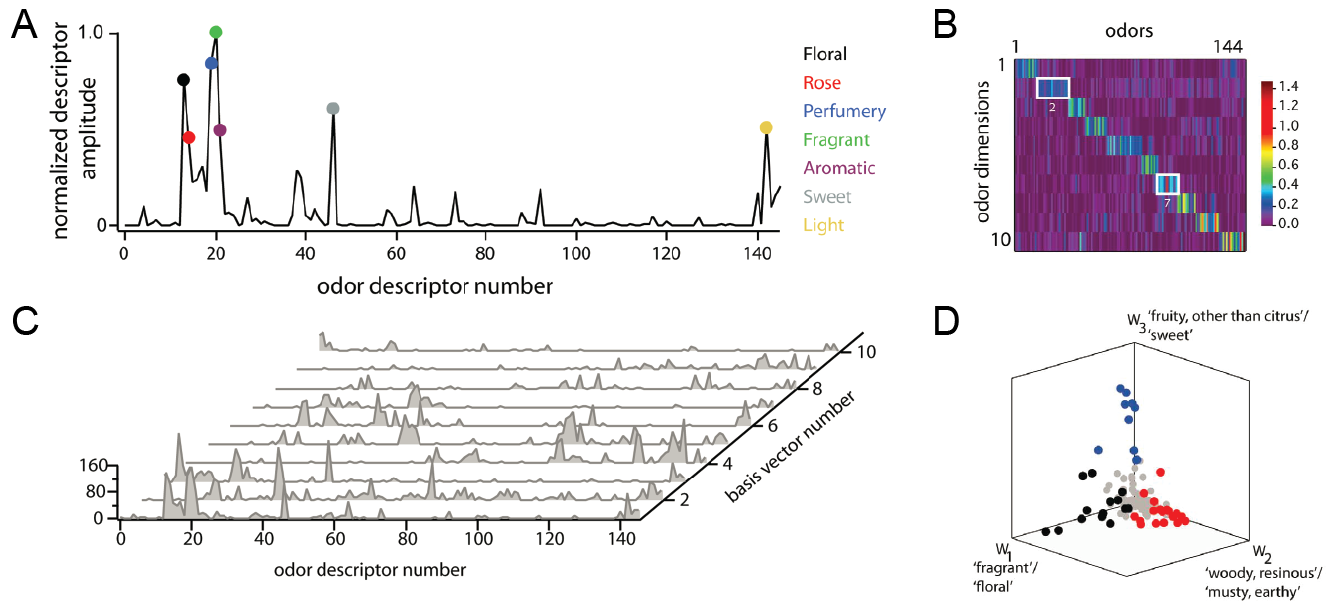
\includegraphics[width=\textwidth]{fig-rev1-olfaction}
    \caption{\revise{\ac{NMF} recovers a sparse and parts-based representation
    of olfactory perceptual space (reprinted from \cite{Castro2013}).
       \textbf{\emph{A}},
          Plot of normalized odor descriptor amplitude vs. odor descriptor number for
          the first basis function. Each point along the x-axis corresponds to a single
          odor descriptor, and the amplitude of each descriptor indicates the
          descriptor's relevance to the shown perceptual basis function.
          Colored circles show the 7 largest elements, with corresponding descriptors
          listed on the right.
       \textbf{\emph{B}},
          Waterfall plot of the 10 basis functions constituting \textbf{W}.
       \textbf{\emph{C}},
          Heat map of the coefficient matrix, \textbf{H},
          where each column of \textbf{H} corresponds to a different odor.
          Columns of \textbf{H} are normalized and sorted into groups defined by
          peak coordinate (1-10).
       \textbf{\emph{D}},
          Plot of all 144 odors in the dataset (each point is a column in \textbf{H})
          in the space spanned by the first three basis functions.
          Black, red, and blue points are those with peak coordinates in dimensions
          1, 2, and 3, respectively. Gray points are all remaining odors.}}
	\label{fig:evidence-olfaction}
\end{figure}

\revise{Castro and colleagues \cite{Castro2013} provided 
one of the most compelling pieces of evidence for \ac{NSC}
in the olfactory system to date:
In an effort to elucidate the dimensions along which perceptual space might be
organized in the olfactory system,
they applied \ac{NMF} to a dataset of 144 monomolecular odors,
each represented by a 146-dimensional odor profile.
Each dimension in the odor profile corresponded to the rated applicability of
a number of semantic labels, such as `sweet', `floral', and `heavy'
(Fig.~\ref{fig:evidence-olfaction}A).
By applying \ac{NMF} to the odor profile, they showed that a small, sparsely active set of basis functions could accurately describe any odor in the dataset
(Fig.~\ref{fig:evidence-olfaction}C).
Interestingly, \ac{NMF} revealed a prominent block
diagonal structure to the full matrix \textbf{H}
(Fig.~\ref{fig:evidence-olfaction}B), indicating that:
1) a given odor tended to be characterized by a single prominent dimension,
implying that the basis functions recovered by \ac{NMF} were perceptually meaningful,
and 2) all 10 dimensions were occupied,
implying that the basis functions recovered by \ac{NMF} could span the space of
behaviorally relevant odors.
This suggests that a given odor percept may be considered an 
instance of one of several fundamental qualities.
For the data set investigated, individual odor profiles were well-classified 
by their proximity to a single one of these dimensions, 
with all ten dimensions being approximately equally expressed 
across the set of odors.}

\revise{Furthermore, \ac{NMF} recovered basis functions whose descriptors align
with perceptual dimensions highlighted in several previous analyses of odor space,
including but not limited to relative pleasantness (e.g., `fragrant`, `sickening`), 
and potential palatability (`woody, resinous', `chemical', `sweet', and `lemon').
Odors clustered predominantly along these axes
(Fig.~\ref{fig:evidence-olfaction}D), 
motivating the interpretation that odor space is organized 
by a relatively large number of independent qualities that apply categorically
\cite{Castro2013}.}


\subsection*{\revise{NSC in the somatosensory cortex}}

\revise{Of all of the sensory areas,
\mikeNote{I rewrote this section to focus on the models}
somatosensory cortex is among the best understood in terms of circuitry,
yet least understood in terms of sensory function
\cite{Ramirez2014}.
Spatiotemporal receptive fields indicate that individual neurons respond to a small number of stimulus dimensions, suggesting a role for dimensionality reduction in primary somatosensory cortex \cite{Ramirez2014}.
In an effort to elucidate the stimulus dimensions that individual neurons respond to,
Whiteway and Butts \cite{WhitewayButts2017} devised the \ac{RLVM},
a combination of nonlinear dimensionality reduction with nonnegativity constraints
that is closely related to \ac{NSC}.
When they applied the \ac{RLVM} to 
a two-photon imaging dataset of hundreds of simultaneously recorded neurons 
in mouse primary somatosensory cortex while the animal was performing
a tactile discrimination task,
they found basis functions that properly identified individual neurons.
Similar to the recorded neuronal responses, these basis functions were closely related
to both the tactile stimulation as well as 
nonstimulus aspects of the behavioral task.
Furthermore, \ac{RLVM} achieved a lower reconstruction error than other
linear dimensionality reduction techniques such as \textbf{\ac{PCA}}.}

\revise{Similar to auditory cortex,
activity in somatosensory cortex can be extremely sparse
\cite{Jadhav2009,oconnor2010,Crochet2011},
and sparse coding models have successfully explained the response properties
of individual neurons in rat somatosensory cortex (e.g., \cite{Hafner2004}).
In addition, the presence of a topographically organized sensory `homunculus' 
in various species \cite{penfield1937,hari1993,petersen2007} 
suggests a possible parts-based representation scheme.}


% \mikeNote{TODO This section needs to discuss at least one NSC modeling paper. That paper should also go in Table 1.}
% \revise{Evidence for a \ac{NSC} mechanism in somatosensory cortex exists for multiple species. First, the presence of a topographically organized sensory `homunculus' in human and bat somatosensory cortex (as well as rat somatosensory, or barrel, cortex) \cite{penfield1937,hari1993,chadha2011,petersen2007} suggests a possible parts-based representation scheme. Second, sparse and efficient coding schemes have been observed in mouse barrel cortex (in one study, 10\% of recorded neurons were active for 50\% of all recorded spikes) \cite{oconnor2010}, with heightened sparsity in an associative fear learning task \cite{gdalyahu2012}. Finally, something akin to mixed selectivity may also be utilized in human somatosensory cortex, according to a non-invasive neuromagnetic imaging study of a high-precision motor task (handwriting). The data suggested rapid modulation of task-specific involvement of somatosensory neurons might be due to the dynamic online selection of pre-existing somatosensory maps \cite{braun2001}. This is further supported by the presence of converging multimodal inputs from disparate regions to somatosensory cortex as observed in cats\cite{kang1985}.}



% \subsection*{\revise{Gustatory cortex}}
% \mikeNote{After a long back and forth, I am against this section. OK it looks intriguing because of similarity to olfactory and parietal cortex, but it's a blue ocean. We don't know anything. There are no models. Why waste space on it?}
% \revise{Despite its similarities to information processing 
% in the olfactory system and parietal cortex,
% gustatory cortex has received relatively little attention
% from an \ac{NSC} viewpoint.
% Gustatory cortex is a multimodal brain region that integrates olfactory
% as well as somatosensory information \cite{DeAraujo2009}
% to give rise to several classes of taste quality
% (e.g., sweet, salty, bitter, sour, umami) \cite{lemon2007}.
% Reminiscent of odor processing in the olfactory bulb,
% taste receptor cells are selective for different classes of chemicals,
% with gustatory fibers maintaining a high degree of specificity
% when carrying taste information into the brain \cite{smith2008central}.
% This functional segregation suggests the existence 
% of a parts-based representation of taste quality.
% Furthermore, taste representations in the gustatory system rely on 
% precise spike time coding \cite{lemon2007},
% suggesting that taste is encoded using a sparse code.
% However, more research is needed to elucidate the underlying coding principles.
% }




\subsection*{\revise{NSC in the retrosplenial cortex (RSC)}}

\revise{In our own work, we found evidence that \ac{NSC} 
\mikeNote{I rewrote this section according to Jeff's comments. I also cleaned up the Supplementary Material section that goes with it: \url{https://www.overleaf.com/14845971vfscrbyrrgrm}}
can explain response properties in \ac{RSC}, 
an area important for navigation and spatial memory 
\cite{Miller2014,Nelson2015,VannAggleton2009}.
Using a similar methodology to \cite{Beyeler2016},
we applied \ac{NMF}, with a sparsity constraint,
to parameterized behavioral variables extracted from electrophyisiological recordings
of \ac{RSC} neurons in the rat \cite{AlexanderNitz2015}
while the animal ran back and forth a W-shaped track
(for experimental details, see Supplementary Material).
As mentioned above, these behavioral variables included the animal's position, head direction, 
and movement direction (Fig.~\ref{fig:NMF|reconstruction}C).
The basis functions recovered by \ac{NMF} were then used to generate simulated responses
of model \ac{RSC} neurons according to Eq.~\ref{eqn:nsc-model-response},
and the simulated responses were compared to neuronal responses 
from the electrophysiological recordings.}

\revise{We found that the population activity of these simulated neurons could be used to predict
the animal's location both with respect to the beginning of the route
(route-based reference frame)
and with respect to where the route was located within the room
(allocentric reference frame).
In addition, simulated neuronal activity could be classified into three broad categories,
with remarkably similar population statistics to rat \ac{RSC}:
1) responding to left and right turns on a specific position along the route,
2) responding to left and right turns regardless the position along the route,
and 3) exhibiting complex and robust firing patterns without turn sensitivity
(see Supplementary Material; also Fig.~\ref{fig:NMF|RSC}A, B).}



% \revise{There is increasing evidence that \ac{NSC} can also explain 
% response properties in \ac{RSC}, .
% As mentioned above, neurons in the \ac{RSC} conjunctively encode multiple variables related to the environment and one's position and movement within it, allowing for the representation of environmental features with respect to multiple spatial reference frames \cite{AlexanderNitz2015}. The \ac{RSC} may also conjunctively encode information about reward in combination with navigation and spatial information \cite{vedder2016}.}
% \mikeNote{We already said all this}

% \revise{In the present paper, 
% we applied NMF to the behavioral data from the original
% \ac{RSC} experiment conducted by Alexander and Nitz \cite{AlexanderNitz2015}
% (for experimental details, see Supplementary Materials).
% \jeffNote{This section is confusing.  There were no neurons in the the NMF application to RSC. I re-wrote the first paragraph, but I am not sure where those numbers are coming from in the second paragraph. }
% \emilyNote{Which numbers, specifically, are confusing? - We had 417 model inputs, we applied NMF and got 30 basis vectors back. Each input reconstruction used 3 or 4 maximally active basis units (which is roughly 10\%). - Because the sparseness of the code means nothing without a comparison, I looked at statistics in the experimental RSC data, found that if you look at the average FR per neuron across trials, 29\% of cells are active. If you look for neurons that fire > 3Hz at least once over the course of a trial, it's more like 50\% active. If you look at response on a bin-by-bin basis (which would be combinations of inputs, the same way we evaluate NMF reconstruction, it's 16\%.}
% Using this method, we were able to reduce the dimensionality of the input space from 417 behavioral inputs to 30 basis functions, and found a close correspondence to the functional patterns of activation between the basis units and the patterns observed in the dataset. Additionally, activity computed from the basis units could be used to replicate the population behavior of the dataset.}
% \revise{We also considered the sparsity of activity in both the experimental data and our model. In the experimental dataset, we found that only 16.3\% of neurons were active for each combination of inputs, while in the \ac{NMF} model, approximately 10\% of the model units (ranging from 3 to 4 out of 30) were active per stimulus combination. Sparse representations of spatial context in the retrosplenial cortex have also been reported elsewhere \cite{mao2017}.} 
% \mikeNote{I removed this because Jeff didn't seem convinced. It would make more sense to measure sparsity using Vinje and Gallant's metric, which talks about population and lifetime sparsity. Then you don't need an arbitrary threshold (3 Hz). However, Reviewer 1 doesn't like lifetime sparsity, so it's best not to go there.}




\subsection*{\revise{Reinforcement-driven NSC in the basal ganglia}}
% \emilyNote{We need to be careful about saying this is direct evidence for NSC, because the proposed mechanism of dimensionality reduction in the basal ganglia is a combination of unsupervised and reinforcement learning. Our flavor of NSC says nothing about reward-driven dimensionality reduction.}
% \mikeNote{The difference is simply that ``this leads to a network that does not simply encode the maximal variability of its input space but rather encodes the variability of the reward-distorted space.'' The reward signal just tells you when to apply the function (dim.red.) - in that sense it's like DA mediating STDP.}
\revise{There is computational evidence 
\mikeNote{shortened, tightened}
for a reward-driven variant of \ac{NSC} in the basal ganglia, 
a cluster of deep forebrain nuclei that are involved in the 
processing of motor, associative, and limbic information
(for recent reviews see \cite{BarGad2003_Review,NelsonKreitzer2014}).
The basal ganglia connect most cortical areas to the frontal cortex through
a series of convergent and sparsely connected pathways \cite{schwab2015},
where signals from tens of millions of cortical neurons are projected
onto a $10 - 10,000$ fold smaller population of neurons in different subnuclei
of the basal ganglia \cite{BarGad2003_Review}.}

\revise{The \ac{RDDR} model suggests that dimensionality reduction 
in the cortico-basal ganglia pathway is achieved via
a combination of Hebbian and anti-Hebbian learning rules
that are implemented by feedforward excitatory and lateral inhibitory
connections \cite{BarGad2000,BarGad2003_Review}.
A reinforcement signal modulates the Hebbian learning rule 
of the feedforward projections,
allowing the network to learn to extract input dimensions
that are associated with reward activity
while suppressing behaviorally irrelevant input dimensions.
Whereas the original \ac{RDDR} model was a neural-network based model
for performing \ac{PCA} \cite{BarGad2000},
later iterations incorporated nonnegativity constraints on the
connection weights that effectively transformed the model 
into an \ac{NMF} variant \cite{BarGad2003_Review}.}

\revise{In addition to suggesting a role for lateral connectivity
in the basal ganglia,
the \ac{RDDR} model also advanced understanding of basal ganglia dysfunction
in movement-related disorders such as Parkinon's and Huntington's disease.
Through a series of simulations, Bar-Gad and colleagues \cite{BarGad2003_Review}
argued that focal lesions should have little effect on behavior,
because of the network's ability to reorganize connections,
whereas abnormal dopamine levels should significantly alter 
the reinforcement signal that controls the model's ability 
to discriminate behaviorally relevant input signals.}


% The RDDR model advanced understanding of the cortico-striato-pallidal loop by clarifying the presence of apparently obsolete lateral connectivity in the basal ganglia and by accounting for previously unexplained experimental findings in patients with diseases associated with the basal ganglia, such as Parkinson's and Huntington's disease.
% This computational model of the basal ganglia is informed by the notion that the role of the basal ganglia is to connect the rest of the cortex to the frontal cortex via the efficient extraction and representation of cortical information used by the frontal cortex for planning upcoming actions \cite{BarGad2000}. It is motivated by the observation that although neuronal activity in the basal ganglia is uncorrelated, this is contradicted by the presence of extensive convergence and lateral inhibitory connections. This hypothesis is tested using a neural network that incorporates key features of the structure of the basal ganglia. It is a multi-layer feedforward network with convergent input and lateral inhibition, featuring Hebbian learning on the feedforward connections and anti-Hebbian learning on the lateral connections. Dimensionality reduction is achieved via the lateral inhibitory connections, which perform PCA (in a subsequent modified model, nonnegativity was enforced on the connections, effectively converting PCA to \ac{NMF}). The network is presented with a series of input patterns whose elements are correlated, some of which are of behavioral relevance to the model for performing an upcoming action (this s signalled to the network using a reinforcement signal, which interacts with the learning in the middle layer of the network (striatal neurons). The network learns to suppress the extraction and representation of irrelevant input patterns while efficiently extracting the relevant ones. Their simulated experimental results show that the mean reconstruction errors of inputs are high, while the amount of data compression in the model is low initially. Over time, input patterns become decorrelated and mean reconstruction errors of inputs are minimal.

% \revise{The basal ganglia are a cluster of nuclei containing the striatum, globus pallidus, substantia nigra, and the subthalamic nuclei. They play a prominent role in the coordination of movement, and are implicated in movement disorders such as Parkinson's disease \cite{BarGad2003_Review}. Together, the basal ganglia, the thalamus, and the cortex form a sophisticated loop consisting of multiple convergent and sparsely connected feedforward pathways that preserve segregated topography between the various layers and their inputs \cite{BarGad2003_Review}. The RDDR model advanced understanding of the cortico-striato-pallidal loop by clarifying the presence of apparently obsolete lateral connectivity in the basal ganglia and by accounting for previously unexplained experimental findings in patients with diseases associated with the basal ganglia, such as Parkinson's and Huntington's disease.}

% \revise{Motivated by the observation of high convergence ratios between regions, Bar-Gad et al. \cite{BarGad2000,BarGad2003_Review} developed the Reinforcement-Driven Dimensionality Reduction (RDDR) model to explain these highly convergent pathways in terms of performing dimensionality reduction. They successfully used Hebbian learning to reproduce basal ganglia response patterns associated with reward \cite{BarGad2000}, a function associated with cortico-striato-pallidal circuitry. The authors later applied nonnegativity constraints to the Hebbian learning in the model so that it effectively performed \ac{NMF} on its inputs. The model advanced understanding of the cortico-striato-pallidal loop by clarifying the presence of apparently obsolete lateral connectivity in the basal ganglia and by accounting for previously unexplained experimental findings in patients with diseases associated with the basal ganglia, such as Parkinson's and Huntington's disease.}
% \mikeNote{TODO So what does it do? This section needs to be more specific.}
% \emilyNote{should be sufficient now}
% \revise{The authors simulated disorders associated with the basal ganglia, such as Parkinson's, by modeling lesions and dopamine depletion in the network. Results of simulated experiments show that focal lesions in the basal ganglia typically have little effect on behavior (because the network adapts and reorganizes its connections, losing minimal components by maintaining important principal ones), while abnormal dopamine levels have major effects (because altering the reinforcement signal impacts the model's ability to discriminate behaviorally relevant input patterns), and also explains the existence of lateral connections in the basal ganglia that appear to have no purpose (the RDDR model suggests that these are heavily utilized during initial learning, but subsequently become obsolete).
% Thus the RDDR network successfully models the behavior of the circuit while explaining the existence of convergent and lateral connections in the region that other models have historically ignored \cite{BarGad2003_Review}. Furthermore, the model is extendable and can be modified to incorporate other anatomical and functional aspects of the biological basal ganglia.}

% \revise{While it has not been clearly reported whether or not activation patterns throughout the basal ganglia are sparse, the maximal connection probabilities between striatal, pallidal, and thalamic neurons are very low ($<$1\%) \cite{BarGad2003_Review}, which may suggest that neurons are also likely to be sparsely activated, and the activity of spiny neurons in the striatum is reportedly sparse \cite{schwab2015}. Corticostriatal neurons in primary motor cortex also exhibit sparse activity \cite{Turner2000}. Parts-based representations seem to exist in the basal ganglia based on the observation of topographical preservation of the kinds of information transmitted in the basal ganglia. The authors note this with respect to their model, saying that nonnegative matrix factorization provides an encoding more consistent with the topographic innervation and sparse encoding of the basal ganglia \cite{BarGad2003_Review}.}



\subsection*{\revise{Potential for NSC in other regions of the brain}}

\revise{In addition to the areas highlighted above,
\mikeNote{Combined unconvincing sections into one}
there is increasing evidence that the essential components of \ac{NSC}
might be present in numerous brain regions 
not traditionally associated with the efficient encoding of information.}

\revise{For example, there is evidence for sparse coding in the
cerebellum \cite{Marr1969,Schweighofer2001,Brunel2004},
\ac{PFC} \cite{Abeles1990,Fujisawa2008,Wei2015},
motor cortex \cite{Beloozerova2003,Kakei2003,BarthPoulet2012,Brecht2004},
hippocampus \cite{rolls2013,ThompsonBest1989,Poli2017,Wixted2014},
and the amygdala \cite{Bach2011}.
Similarly, there is evidence for dimensionality reduction at least in
\ac{PFC} \cite{Mante2013}
and motor cortex \cite{Graziano2009,Gallego2017}.
However, the intrinsically complex response properties of individual neurons
have defied a deep understanding of how these neurons contribute to behavior
\cite{churchland2007,Mante2013}.
For example, individual \ac{PFC} neurons typically encode multiple task-related signals
at once, including the animal's upcoming choice, the context,
and the strength of the sensory evidence \cite{Mante2013,Rigotti2013,Kobak2016}.
Future studies may show that key features of the population response in these regions
can be recovered by applying \ac{NSC} to their inputs.}

\revise{Analogous to our modeling work in \ac{MSTd} \cite{Beyeler2016},
it might be possible to apply \ac{NSC} to other areas of the posterior parietal
cortex that are involved in multisensory heading perception.
Areas such as the \ac{VIP} and \ac{VPS} are also known to respond to optic flow,
but they increasingly respond to inertial vestibular stimulation as well
\cite{Chen2011}.
Although the sparseness of the population code in \ac{VIP} and \ac{VPS} is not known,
the fact that neurons in these areas respond to mixtures of visual and vestibular
heading cues make them prime examples 
to be examined with an \ac{NSC} based modeling approach.}

\revise{Elsewhere in parietal cortex, single neurons act as basis functions 
to represent the spatial configuration of objects 
with respect to multiple reference frames
(e.g., by transforming eye-centered to body-centered coordinates).
\cite{Poggio1990,PougetSejnowski1997,PougetSnyder2000}.
This is similar to the integration of multimodal heading cues mentioned above,
as well as to other associative areas such as \ac{RSC},
which demonstrates conjunctive coding of various spatial navigation cues
\cite{AlexanderNitz2015,Rounds2018}.
There is further evidence that actions are represented in parietal cortex
with respect to arbitrary and abstract reference frames, 
such as with respect to a planned route through an environment \cite{nitz2009parietal}.
From a theoretical standpoint, \ac{NSC} seems a good candidate to find an efficient,
reference-frame agnostic representation of various behaviorally relevant variables
\cite{LouieGlimcher2012,louie2015adaptive,andersen1997multimodal,BenHamed2003},
but future studies will have to address these issues step by step.}




% \subsection*{\revise{Prefrontal cortex (PFC)}}
% \jeffNote{The first 2 paragraphs say nothing about NMF or NSC.  Is the evidence strong in the PFC?  I would consider deleting this section.}
% \mikeNote{Merge into above / delete}
% \revise{\Ac{PFC} is thought to play a fundamental role in 
% flexible, context-dependent behavior,
% but the exact nature of the computations underlying this role 
% remains large unknown \cite{Mante2013}.
% Individual \ac{PFC} neurons typically encode multiple task-related signals
% at once, including the animal's upcoming choice, the context,
% and the strength of the sensory evidence \cite{Mante2013,Rigotti2013,Kobak2016},
% defying a deep understanding of how 
% individual \ac{PFC} neurons contribute to behavior.
% Researchers have argued that high-dimensional neural representations
% enable simple readout mechanisms such as linear classifiers to implement
% a large set of input-output relations \cite{Rigotti2013,Barak2013}.}

% \revise{The most successful modeling studies in \ac{PFC} have asked
% whether the confounding single-neuron responses could be understood as
% views of a simple dynamical process at the population level
% \cite{Mante2013}.
% They found that \ac{PFC} population responses dynamically encode several task variables underlying an animal's behavior.
% During decision making, the response to a choice stimulus is characterized
% by an initial stimulus-specific population response,
% but evolves to different final decision related
% states depending on the current rule \cite{Stokes2013}.}

% \revise{While there is evidence of dimensionality reduction 
% in \ac{PFC} \cite{Mante2013},
% little is known about the sparsity of the population code.
% The only evidence for sparse coding is restricted to the \ac{mPFC} in rats
% \cite{Fujisawa2008,Wei2015},
% an area that is engaged in working memory tasks 
% and sensitive to the expectation of reward \cite{Baeg2003}.
% Whereas \ac{NMF} was able to elucidate functional properties of the \ac{mPFC}
% network while rats behaved in a Y-maze \cite{Wei2015},
% the study also highlighted the dependence of \ac{mPFC} network activity
% on the animal's choice behavior.}




% \subsection*{\revise{Motor cortex}}
% \jeffNote{Same comment as in PFC.  Just because its sparse or parts-based does not imply NMF or NSC.  This doesn't seem like a strong argument.}
% \mikeNote{Merge into above / delete}
% \revise{As in the somatosensory cortex, there exists a topographic partitioning of 
% representations of the body in the primary motor cortex, referred to as the motor homunculus \cite{penfield1937,metman1993}. This constitutes evidence for the existence of parts-based representations in at least some parts of motor cortex, in combination with studies that show the activity patterns associated with small sets of neurons in primary motor cortex represent naturalistic movements, and can be used to reconstruct joint angles \cite{Vargas2010decoding}. The organization of the motor cortex as it progresses past primary motor is less clear, but some researchers suggest that these regions can be well-described using nearest-neighbor similarity \cite{GrazianoAflalo2007}. They argue that topographical organization is easy to accomplish when the input space to be mapped is two-dimensional like the cortical sheet, but as input spaces become increasingly high-dimensional, topograhic organization disappears as different inputs and combinations of inputs compete for representation. Using a model that was initially organized somatotopically, the researchers studied the self-guided reorganization of the map in response to hand position and a set of movement dimensions that corresponded to those movements a monkey would be physically able to perform. They found that principles of nearest-neighbor similarity described the way that such a high-dimensional space was mapped onto a two-dimensional surface, and which reflected the actual organization of the motor cortex, and was constituted of sets of parts-based representations \cite{GrazianoAflalo2007}.} 

% \revise{This idea also appears to be consistent with the somatosensory and motor representations of arms and movement in octopuses, who do not have topographically organized sensorimotor maps. Instead, their nervous system structure is centralized, with body part and movement representations being highly distributed \cite{zullo2011}. There is a hierarchical organization evident, with highly stereotyped movement circuits at the periphery and distributed but overlapping parallel pathways at the center for higher motor control, which likely integrate sensory inputs. Thus the octopus can efficiently execute commands via the central control pathways that then execute automated movements in the individual arms. This structure and organization appears consistent with the nearest-neighbor similarity concept of organization described by Graziano and Aflalo \cite{GrazianoAflalo2007}.}

% \revise{Evidence for sparse coding in the motor cortex, on the other hand, is lacking---in fact, some studies suggest that most neurons are active in motor cortex during movement preparation and support a basis set by which many movement parameters are represented \cite{churchland2007}.
% The role of neurons that do not explicitly represent any movement parameters
% can be explained by recent work based on optimal feedback control theory, 
% which postulates that the goal of motor cortex is to produce a desired movement and force, taking into account the state of the muscles \cite{Gallego2017}.
% This hypothesis avoids the need for explicit representation 
% of movement parameters covariates by single neurons,
% although some neurons may still represent some movement parameters
% as a byproduct of the necessary control signals
% \cite{Gallego2017}.}


% \subsection*{\revise{Hippocampus}}

% \jeffNote{Same comment as in PFC and motor cortex.  Just because its sparse or parts-based does not imply NMF or NSC.  This doesn't seem like a strong argument. You may want to have a section called "Other areas" that states there is evidence for dimenionality reduction, parts-based representations, and sparse activity in the PFC, motor cortex, and hippocampus. Future studies may show that features can be recovered by applying NSC to the inputs of these regions.}
% \mikeNote{TODO Merge into above / delete}
% \revise{The CA1 region of the hippocampus have long been thought of as an auto-associative network that automatically performs pattern completion in response to partial inputs \cite{rolls2013}, while the dentate gyrus and hippocampal CA3 are believed to perform pattern separation in order to sparsify and decorrelate the entorhinal inputs coming into the hippocampus \cite{Bakker2008}. This orthogonalization of overlapping input patterns is thought to underlie the formation of episodic memories and the discrimination of similar environmental contexts by the hippocampus \cite{myers2011pattern}. Likewise, activity in both the dentate gyrus granule cells and in pyramidal cells in hippocampal CA1/CA3 subfields is sparse \cite{Poli2017}.
% In support of a parts-based representation scheme, hippocampal neurons exhibit conjunctive encoding and mixed selectivity properties similar to those observed in retrosplenial cortex \cite{komorowski2009,mckenzie2014}.}